\chapter{Low-Level Design}
\label{chap:low-level-design}

\section{Introduction}
The Low-Level Design (LLD) provides a detailed, code-adjacent view of the components that make up the Nexus PM platform. It defines the logical structure, internal boundaries, component relationships, data transfer schemas (DTOs), database schemas, and integration logic for every system module. By translating high-level containers and services into detailed component mappings, this chapter serves as the primary technical specification for developers and maintainers of the platform.

The specifications in this chapter are derived directly from the active, production-ready codebase of Nexus PM. The system is designed as a modular monolith, enforcing a strict separation of concerns through layers: Route Handlers (Routers), Service Layers (Business Logic), and the Database Access Layer (Repositories/ORM Models).

\section{Authentication Module}
The Authentication Module is responsible for secure identity assertion, Google OAuth federated login, and stateless user session tracking.

\subsection{Purpose and Responsibilities}
This module processes credentials, generates security tokens, validates third-party authentication signatures, and manages refresh token lifecycles to prevent unauthorized access.

\begin{table}[h!]
\centering
\small
\renewcommand{\arraystretch}{1.4}
\begin{tabularx}{\textwidth}{>{\ttfamily\small}p{4.2cm} X}
    \toprule[1.5pt]
    \rowcolor{primary!5}
    \multicolumn{1}{l}{\textbf{\color{primary}Component}} & \textbf{\color{primary}Technical Responsibility} \\
    \midrule
    \texttt{\detokenize{api/routes/auth.py}} & Exposes endpoints for login, registration, token refresh, and Google OAuth callbacks. \\
    \texttt{\detokenize{services/auth_service.py}} & Coordinates credential hashing checks, maps federated identities, and generates JWT payload signatures. \\
    \texttt{\detokenize{dependencies/auth.py}} & Enforces route protection checks, extracts user records from database sessions using JWT values. \\
    \texttt{\detokenize{models/refresh_token.py}} & Persists active refresh tokens to support session revocation and token-rotation validation. \\
    \bottomrule[1.5pt]
\end{tabularx}
\caption{Authentication Module Component Specifications}
\label{tab:auth_components}
\end{table}

\subsection{Interaction Flow and Data Flow}
When a user initiates local authentication:
\begin{enumerate}
    \item The client issues a HTTP POST request to \path{/api/auth/login} containing the email and password payload.
    \item The router parses the request using the Pydantic \texttt{UserLogin} schema.
    \item The service layer queries the user table, retrieves the matching \texttt{User} record, and verifies the password hash using \texttt{passlib.context} (bcrypt).
    \item Upon validation, the service generates a stateless access token (valid for 15 minutes) containing the user's email in the \texttt{sub} claim, and a random refresh UUID (valid for 7 days) stored in the database.
    \item The tokens are returned to the client, with the refresh token set as a secure, \texttt{HttpOnly} cookie, with SameSite settings defaulting to \texttt{Lax} (or configured via environment variables).
\end{enumerate}

\subsection{Security and Scalability Notes}
\begin{itemize}
    \item \textbf{Token Security:} Session validation is stateless, offloading signature checks from database reads. The system uses SHA256 HMAC algorithms with server keys.
    \item \textbf{Rate Limiting:} To block brute-force attempts, login endpoints are throttled using rate limits tracked in Upstash Redis.
\end{itemize}

\section{User Management Module}
The User Management Module coordinates profile settings, avatar asset mappings, and basic user access controls.

\subsection{Purpose and Responsibilities}
This module enables users to configure profile attributes, handles profile listings for project invitations, and manages the lifecycle of user records.

\begin{table}[h!]
\centering
\small
\renewcommand{\arraystretch}{1.4}
\begin{tabularx}{\textwidth}{>{\ttfamily\small}p{4.2cm} X}
    \toprule[1.5pt]
    \rowcolor{primary!5}
    \multicolumn{1}{l}{\textbf{\color{primary}Component}} & \textbf{\color{primary}Technical Responsibility} \\
    \midrule
    \texttt{\detokenize{api/routes/users.py}} & Exposes endpoints to retrieve current profile parameters, update user settings, and query users by email. \\
    \texttt{\detokenize{schemas/user.py}} & Defines data serialization and validation formats for user requests and updates. \\
    \texttt{\detokenize{models/user.py}} & Implements the SQLAlchemy User model mapped to the primary relational database table. \\
    \bottomrule[1.5pt]
\end{tabularx}
\caption{User Management Module Component Specifications}
\label{tab:user_components}
\end{table}

\subsection{Interaction Flow and Lifecycle}
Profile updates follow a direct path:
\begin{enumerate}
    \item The client submits a PUT request to \path{/api/users/profile} with modified fields (e.g., \texttt{full\_name}, \texttt{avatar\_url}).
    \item The route handler extracts the user profile from the database using the \texttt{get\_current\_user} dependency.
    \item The router validates the input payload against the \texttt{UserUpdate} Pydantic schema.
    \item The database entity is updated, and the transaction is committed, returning the updated user profile model.
\end{enumerate}

\subsection{Security and Scalability Notes}
\begin{itemize}
    \item \textbf{Data Privacy:} Access to sensitive fields (e.g., Google ID, password hashes) is restricted at the API layer by using separate Pydantic output serialization models (\texttt{UserResponse}).
    \item \textbf{Asset Storage Integration:} Avatars are uploaded to Cloudflare R2, storing only the public asset URL in the database user record to avoid database bloat.
\end{itemize}

\section{Project Management Module}
The Project Management Module governs workspace resources, project status tracking, and workspace collaborator roles.

\subsection{Purpose and Responsibilities}
This module manages workspace isolation, project creation, member role assignments, and project metadata serialization.

\begin{table}[h!]
\centering
\small
\renewcommand{\arraystretch}{1.4}
\begin{tabularx}{\textwidth}{>{\ttfamily\small}p{4.2cm} X}
    \toprule[1.5pt]
    \rowcolor{primary!5}
    \multicolumn{1}{l}{\textbf{\color{primary}Component}} & \textbf{\color{primary}Technical Responsibility} \\
    \midrule
    \texttt{\detokenize{api/routes/projects.py}} & Handles project CRUD operations and queries project records within active workspaces. \\
    \texttt{\detokenize{api/routes/project_members.py}} & Exposes endpoints to add project members, update user roles, and accept project invitations. \\
    \texttt{\detokenize{services/project_service.py}} & Implements business logic for project workspace partitioning and project state updates. \\
    \texttt{\detokenize{services/project_member_service.py}} & Enforces role checks, evaluates permission levels, and manages membership transitions. \\
    \bottomrule[1.5pt]
\end{tabularx}
\caption{Project Management Module Component Specifications}
\label{tab:project_components}
\end{table}

\subsection{Interaction Flow and Data Flow}
When adding a member to a project:
\begin{enumerate}
    \item The project administrator submits a POST request to \texttt{/api/projects/\{project\_id\}/members} containing the invitee's email and role.
    \item The system verifies that the inviter has the required permissions (e.g., \texttt{owner} or \texttt{manager}) in the project.
    \item The database is checked for an existing membership record to prevent duplicates.
    \item On validation, the user relation is saved in the \texttt{ProjectMember} association table.
    \item The system triggers a background email notification via the Resend API to alert the user of the project assignment.
\end{enumerate}

\subsection{Security and Scalability Notes}
\begin{itemize}
    \item \textbf{Workspace Isolation:} Database queries restrict access based on active project memberships. This design acts as a core security boundary, preventing data leakage across workspaces.
    \item \textbf{Role-Based Dependency Injection:} Sensitive routes verify roles before executing route handlers by injecting the \texttt{require\_project\_role} helper.
\end{itemize}

\section{Task Management Module}
The Task Management Module manages task workflows, priorities, comment threads, assignments, and due dates.

\subsection{Purpose and Responsibilities}
This module serves as the primary task engine, coordinating task states, due date tracking, comment histories, and board layout configurations.

\begin{table}[h!]
\centering
\small
\renewcommand{\arraystretch}{1.4}
\begin{tabularx}{\textwidth}{>{\ttfamily\small}p{4.2cm} X}
    \toprule[1.5pt]
    \rowcolor{primary!5}
    \multicolumn{1}{l}{\textbf{\color{primary}Component}} & \textbf{\color{primary}Technical Responsibility} \\
    \midrule
    \texttt{\detokenize{api/routes/tasks.py}} & Exposes endpoints for task CRUD operations, status updates, and assignee mappings. \\
    \texttt{\detokenize{api/routes/comments.py}} & Manages comment creation, comment editing, and comment deletion. \\
    \texttt{\detokenize{services/task_service.py}} & Enforces task validation rules, updates priorities, and triggers status changes. \\
    \texttt{\detokenize{services/comment_service.py}} & Manages comments, verifying user edit permissions before database commit. \\
    \bottomrule[1.5pt]
\end{tabularx}
\caption{Task Management Module Component Specifications}
\label{tab:task_components}
\end{table}

\subsection{Interaction Flow and Data Flow}
When a user updates a task status on the Kanban board:
\begin{enumerate}
    \item The client issues a PUT request to \path{/api/tasks/{task_id}} with the updated status lane (e.g., \texttt{IN\_PROGRESS}).
    \item The backend route handler intercepts the request, verifying the user's role access for the parent project.
    \item The service layer retrieves the task entity and updates the status attribute.
    \item The service appends an audit event to the \texttt{ActivityLog} table.
    \item The database commit completes, and the updated task details are returned to refresh the client interface.
\end{enumerate}

\subsection{Security and Scalability Notes}
\begin{itemize}
    \item \textbf{Cascading Deletes:} Task deletion automatically triggers cascade deletes for associated comment threads and task attachment records, preventing orphaned database records.
    \item \textbf{Index Optimization:} Database indexes are configured on \texttt{project\_id} and \texttt{assigned\_to} columns to ensure fast search performance as database size grows.
\end{itemize}

\section{Storage Module}
The Storage Module manages file attachments, pre-signed upload URLs, and asset access control.

\subsection{Purpose and Responsibilities}
This module handles file uploads by coordinating with Cloudflare R2, validating file sizes and MIME types, and managing database attachment records.

\begin{table}[h!]
\centering
\small
\renewcommand{\arraystretch}{1.4}
\begin{tabularx}{\textwidth}{>{\ttfamily\small}p{4.2cm} X}
    \toprule[1.5pt]
    \rowcolor{primary!5}
    \multicolumn{1}{l}{\textbf{\color{primary}Component}} & \textbf{\color{primary}Technical Responsibility} \\
    \midrule
    \texttt{\detokenize{api/routes/storage.py}} & Exposes endpoints for pre-signed upload URL requests and attachment registrations. \\
    \texttt{\detokenize{services/storage_service.py}} & Interfaces with Cloudflare R2 using AWS SDK clients to generate short-lived upload URLs. \\
    \texttt{\detokenize{services/task_attachment_service.py}} & Manages attachment records in PostgreSQL and links uploaded files to tasks. \\
    \texttt{\detokenize{models/task_attachment.py}} & Defines metadata structures (file key, size, type, URL) for uploaded assets. \\
    \bottomrule[1.5pt]
\end{tabularx}
\caption{Storage Module Component Specifications}
\label{tab:storage_components}
\end{table}

\subsection{Interaction Flow and Data Flow}
To ensure secure and efficient file uploads:
\begin{enumerate}
    \item The client requests a pre-signed URL by issuing a POST request to \path{/api/storage/presigned-url} containing the filename, size, and MIME type.
    \item The backend validates that the file size is under limits (e.g., 10MB) and the MIME type is in the whitelist.
    \item The storage service contacts the Cloudflare R2 API to generate a pre-signed PUT URL valid for 15 minutes.
    \item The pre-signed URL is returned to the client, which uploads the file stream directly to R2, bypassing backend compute overhead.
    \item Once the upload completes, the client registers the attachment metadata with the backend, linking it to the corresponding task entity.
\end{enumerate}

\subsection{Security and Scalability Notes}
\begin{itemize}
    \item \textbf{Zero Backend Storage Overhead:} Offloading file streams directly to R2 prevents backend thread blocks and reduces API egress costs.
    \item \textbf{Validation Policies:} Whitelist validation prevents users from uploading executable files or scripts that could target client browsers.
\end{itemize}

\begin{figure}[h!]
    \centering
    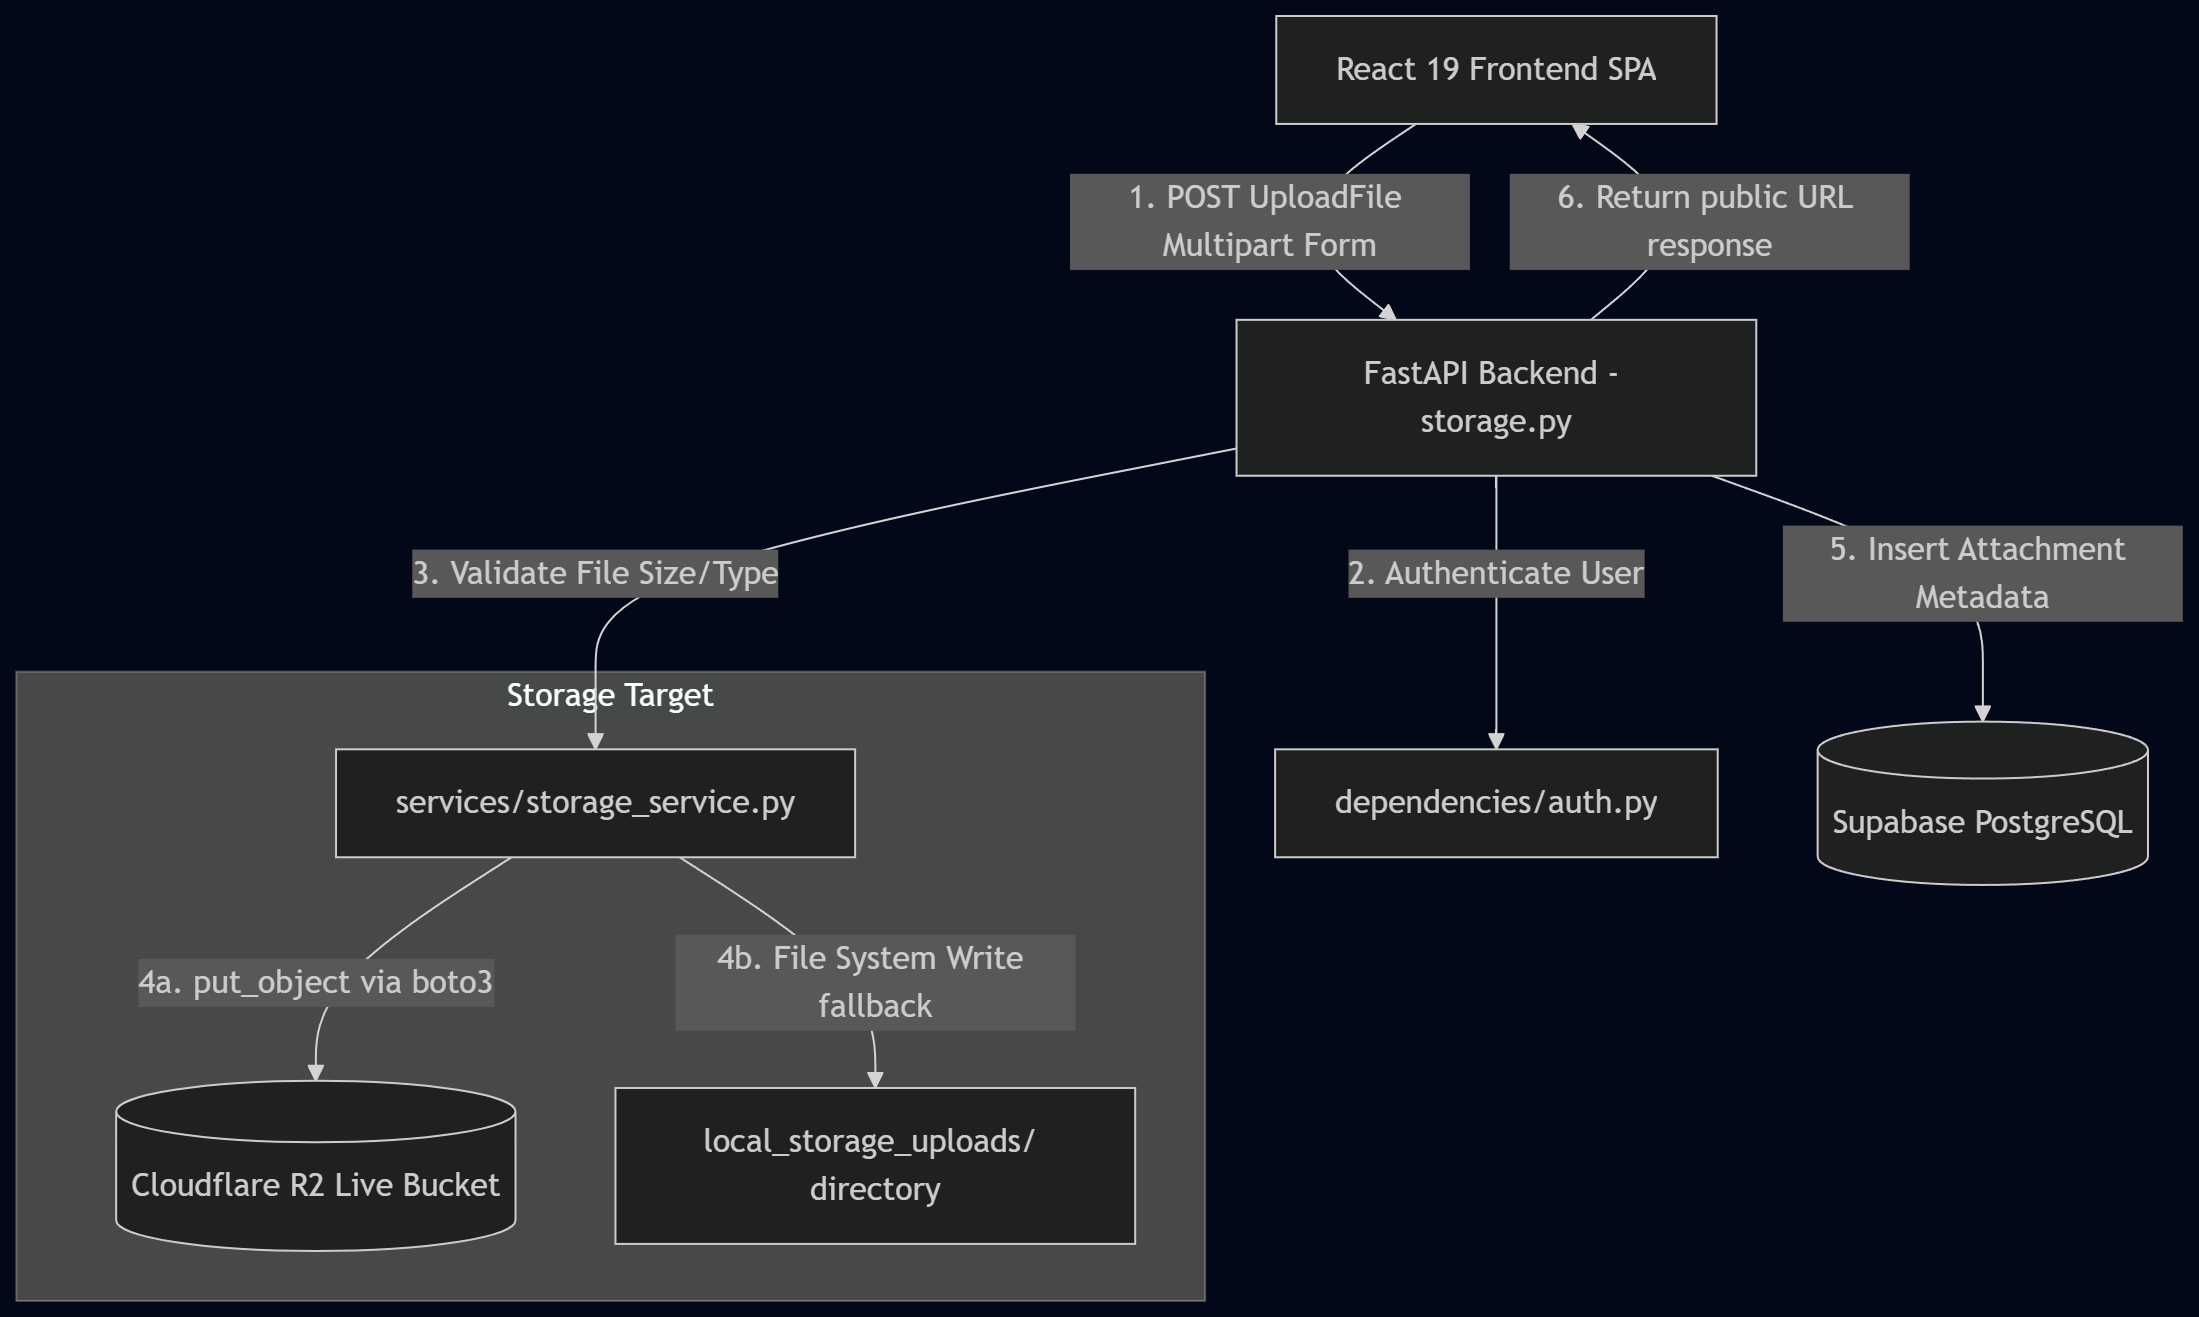
\includegraphics[width=\textwidth]{figures/storage-architecture.png}
    \caption{Nexus PM S3-Compatible Storage Direct Upload Flow}
    \label{fig:storage_flow_diagram}
\end{figure}

\section{Notification Module}
The Notification Module manages in-app alerts, read status tracking, and transactional email dispatches.

\subsection{Purpose and Responsibilities}
This module monitors project events, registers in-app notification records, handles unread counters, and dispatches external email alerts.

\begin{table}[h!]
\centering
\small
\renewcommand{\arraystretch}{1.4}
\begin{tabularx}{\textwidth}{>{\ttfamily\small}p{4.2cm} X}
    \toprule[1.5pt]
    \rowcolor{primary!5}
    \multicolumn{1}{l}{\textbf{\color{primary}Component}} & \textbf{\color{primary}Technical Responsibility} \\
    \midrule
    \texttt{\detokenize{api/routes/notifications.py}} & Exposes endpoints to fetch notifications, mark alerts as read, and retrieve unread counts. \\
    \texttt{\detokenize{services/notification_service.py}} & Handles the creation of notification records and evaluates user subscription rules. \\
    \texttt{\detokenize{services/email.py}} & Interfaces with the Resend API to construct and dispatch HTML transactional emails. \\
    \texttt{\detokenize{models/notification.py}} & Stores notification details (recipient ID, event type, message, read state) in PostgreSQL. \\
    \bottomrule[1.5pt]
\end{tabularx}
\caption{Notification Module Component Specifications}
\label{tab:notification_components}
\end{table}

\subsection{Interaction Flow and Data Flow}
When a user triggers a notification event (e.g., task assignment):
\begin{enumerate}
    \item The task service creates the task assignment and calls the notification service with the recipient and task details.
    \item The notification service creates an in-app alert record in the database.
    \item The notification service triggers a background worker to call the email service.
    \item The email service builds the HTML email template and sends it to the Resend API gateway.
    \item The client updates the unread badge count via database query polling.
\end{enumerate}

\subsection{Security and Scalability Notes}
\begin{itemize}
    \item \textbf{Asynchronous Email Processing:} Running email API dispatches in background threads prevents external network delays from slowing backend API response times.
    \item \textbf{Recipient Access Validation:} Notification updates require recipient ID validation to ensure users can only modify their own notification status.
\end{itemize}

\section{Analytics Module}
The Analytics Module computes project metrics and progress analytics to populate the user dashboard.

\subsection{Purpose and Responsibilities}
This module calculates database statistics, groups task states, aggregates member workloads, and generates project progress metrics.

\begin{table}[h!]
\centering
\small
\renewcommand{\arraystretch}{1.4}
\begin{tabularx}{\textwidth}{>{\ttfamily\small}p{4.2cm} X}
    \toprule[1.5pt]
    \rowcolor{primary!5}
    \multicolumn{1}{l}{\textbf{\color{primary}Component}} & \textbf{\color{primary}Technical Responsibility} \\
    \midrule
    \texttt{\detokenize{api/routes/analytics.py}} & Exposes API endpoints for retrieving workspace and project metrics. \\
    \texttt{\detokenize{services/analytics_service.py}} & Implements optimized database queries to aggregate task counts, completion states, and timeline trends. \\
    \bottomrule[1.5pt]
\end{tabularx}
\caption{Analytics Module Component Specifications}
\label{tab:analytics_components}
\end{table}

\subsection{Interaction Flow and Data Flow}
When a user opens the workspace dashboard:
\begin{enumerate}
    \item The client issues a GET request to \texttt{/api/analytics/workspace/\{workspace\_id\}}.
    \item The route handler validates that the user is an active workspace member.
    \item The service executes aggregated database queries, calculating total open tasks, tasks in progress, completed tasks, and average cycle times.
    \item The service caches the calculated JSON payload in Upstash Redis with a 5-minute expiration window to reduce database load.
    \item The aggregated data is returned to the client to render the dashboard layout.
\end{enumerate}

\subsection{Security and Scalability Notes}
\begin{itemize}
    \item \textbf{Aggregated Cache Validation:} Caching analytical queries prevents resource-intensive database calculations on every page view.
    \item \textbf{Read-Only Optimization:} Database queries use readonly, index-supported executions to optimize performance.
\end{itemize}

\section{AI Module}
The AI Module coordinates with Google Gemini to generate task suggestions and project updates.

\subsection{Purpose and Responsibilities}
This module constructs prompt templates, invokes the Gemini API, parses generated JSON outputs, and validates AI response structures.

\begin{table}[h!]
\centering
\small
\renewcommand{\arraystretch}{1.4}
\begin{tabularx}{\textwidth}{>{\ttfamily\small}p{4.2cm} X}
    \toprule[1.5pt]
    \rowcolor{primary!5}
    \multicolumn{1}{l}{\textbf{\color{primary}Component}} & \textbf{\color{primary}Technical Responsibility} \\
    \midrule
    \texttt{\detokenize{api/routes/ai.py}} & Exposes API routes for task decomposition, meeting note parsing, and project status updates. \\
    \texttt{\detokenize{services/ai_service.py}} & Manages the GenAI client connection, handles API errors, and manages model parameter configs. \\
    \bottomrule[1.5pt]
\end{tabularx}
\caption{AI Module Component Specifications}
\label{tab:ai_components}
\end{table}

\subsection{Interaction Flow and Data Flow}
When task decomposition is triggered:
\begin{enumerate}
    \item The client submits a POST request to the task generation endpoint with the target project ID.
    \item The router checks the user's project role and retrieves the project description from the database.
    \item The AI component builds the context payload and defines a system instruction requesting a structured JSON array.
    \item The service calls the Gemini 2.5 Flash model asynchronously using the GenAI client.
    \item The model returns the text block. The AI component extracts the JSON array, parses it, and validates it against the schema.
    \item The sub-tasks are created in the database, and the updated task structure is returned to the client.
\end{enumerate}

\subsection{Security and Scalability Notes}
\begin{itemize}
    \item \textbf{Structured Output Validation:} Sanitizing and validating the model's text output prevents malformed JSON strings from causing application parsing failures.
    \item \textbf{Error and Rate Limit Handling:} The service handles rate limiting (HTTP 429) and timeout errors (HTTP 504) from the Gemini API, returning user-friendly error messages and preventing transaction failures.
\end{itemize}

\section{Database Layer}
The Database Layer manages connection setups, SQLAlchemy configurations, transaction cycles, and migration versions.

\subsection{Purpose and Responsibilities}
This layer provides database connection management, coordinates migrations, and manages query executions.

\begin{table}[h!]
\centering
\small
\renewcommand{\arraystretch}{1.4}
\begin{tabularx}{\textwidth}{>{\ttfamily\small}p{4.2cm} X}
    \toprule[1.5pt]
    \rowcolor{primary!5}
    \multicolumn{1}{l}{\textbf{\color{primary}Component}} & \textbf{\color{primary}Technical Responsibility} \\
    \midrule
    \texttt{\detokenize{db/database.py}} & Establishes the asynchronous engine, configures connection parameters, and manages connection pools. \\
    \texttt{\detokenize{db/base.py}} & References all database models to ensure proper schema generation by Alembic. \\
    \texttt{\detokenize{alembic.ini}} & Configures migration directories, logging, and database targets. \\
    \bottomrule[1.5pt]
\end{tabularx}
\caption{Database Layer Component Specifications}
\label{tab:db_components}
\end{table}

\subsection{Connection Pool and PgBouncer Specifications}
The database engine is configured to ensure optimal performance within free-tier limits:
\begin{itemize}
    \item \textbf{Async Connection Pool:} The engine uses \texttt{create\_async\_engine} with \texttt{pool\_pre\_ping=True} to verify connections before executing queries, preventing failures on dead connections.
    \item \textbf{PgBouncer Connection Pooling:} Supabase handles connection routing through PgBouncer, resolving database connection limits. The engine disables the local statement cache (\texttt{"statement\_cache\_size": 0}) to avoid conflicts with PgBouncer's transaction mode.
\end{itemize}

\section{External Services}
Nexus PM integrates with several external services to simplify infrastructure requirements and maintain a low operational footprint:

\begin{itemize}
    \item \textbf{Supabase (PostgreSQL):} Serves as the primary transactional database, providing managed PostgreSQL tables, connection pooling, and automatic backups.
    \item \textbf{Cloudflare R2:} Handles file attachments, eliminating local file storage requirements and providing S3-compatible asset management with zero data egress costs.
    \item \textbf{Upstash Redis:} Provides a serverless cache layer for rate limiting, session storage, and analytical query caching, scaling dynamically based on traffic volume.
    \item \textbf{Resend:} Handles transactional email delivery via API, providing high deliverability and simple integration.
    \item \textbf{Google OAuth:} Delegates authentication security to Google's sign-in infrastructure, avoiding the risks of storing user credentials locally.
    \item \textbf{Google Gemini API Gateway:} Integrates Large Language Model capabilities, returning structured JSON response payloads based on prompt variables.
\end{itemize}

\section{Chapter Summary}
This chapter detailed the Low-Level Design of the Nexus PM platform, specifying component dependencies, interaction lifecycles, and security controls for all core modules. By documenting database schemas, API parameters, and integration configurations, this design provides a clear reference for the development and maintenance of the codebase. The following chapters will outline the testing protocols, deployment designs, and validation checks used to verify this implementation.
